\documentclass[10pt,firamath,cours]{nsi}
\begin{document}

\chapter{Arbres binaires}
\section{Généralités}
\subsection{Arbres}
La structure d'arbre n'est pas linéaire : les éléments n'y sont pas rangés les uns à la suite des autres.
C'est une structure \textit{hiérarchique} : les éléments y sont organisés en \textit{niveaux}.\\

Dans ce chapitre nous étudions les \textit{arbres binaires}.


\begin{definition}[s : arbre binaire, sous-arbre, racine]
    \picleft{0.5}{img/arbre_bin_1}{
        Un arbre binaire peut être vide.
        Sinon, il est composé d'au moins un n\oe ud, appelé \textit{racine} et le reste des n\oe uds peut être partagé en 2 sous-ensembles : le \textit{sous-arbre gauche} et le \textit{sous-arbre droit}.
        
        Un n\oe ud possède toujours un sous-arbre droit et un sous-arbre gauche, même si ceux-ci peuvent être vides (segments gris en pointillés).  }
\end{definition}



\begin{definition}[ : fils]
    \picright{0.5}{img/arbre_bin_2}{
        Quand le sous-arbre gauche d'un n\oe ud est non-vide, sa racine est appelée \textit{fils gauche} du n\oe ud. On définit de même la notion de \textit{fils droit}.
    }
\end{definition}

\begin{definition}[ : taille]
    \picleft{0.3}{img/arbre_bin_5}{
        La \textit{taille} d'un arbre est le nombre de ses n\oe uds.
        Voici un arbre de taille 8.}
\end{definition}

\begin{definition}[ : hauteur et feuille]
    \picright{0.3}{img/arbre_bin_3}{
        On appelle \textit{feuille} tout n\oe ud qui n'a ni fils droit ni fils gauche.\\
        La \textit{hauteur} d'un n\oe ud est le nombre d'arêtes qui mène de la racine à ce n\oe ud).\\
        La hauteur de l'arbre est la plus grande des hauteurs des n\oe uds qui le composent.\\
        Cet arbre est de hauteur 3.}
\end{definition}

\begin{remarque}[]
    La définition de hauteur \textit{ n'est pas standard}. Selon celle-ci la hauteur de l'arbre vide n'est pas définie.\\
    
    On choisit parfois de définir la hauteur d'un n\oe ud comme le nombre de n\oe uds pour aller jusqu'à la racine incluse, et on fixe la hauteur de l'arbre vide à zéro.\\
    
    Cela donne une hauteur qui est supérieure d'une unité par rapport à celle choisie dans ce cours.   
\end{remarque}


\begin{definition}[ : n\oe ud interne, arbre dégénéré]
    \picright{0.3}{img/peigne}{
        Un n\oe ud qui n'est ni la racine ni une feuille est dit \textit{interne}.\\
        
        Si tous les n\oe uds internes n'ont qu'un seul fils, l'arbre est dit \textit{dégénéré}.
    }
\end{definition}
\begin{definition}[ : arbre parfait]
    \picleft{0.3}{img/parfait}{
        Si tous les n\oe uds internes ont 2 fils et que toutes les feuilles sont à la même hauteur, on dit que l'arbre binaire est \textit{parfait}.
        
    }
\end{definition}






\section{Structure de données}
\subsection{Modèle théorique}
\begin{encadrecolore}{Interface théorique}{UGLiGreen}
    \begin{itemize}
        \item \textit{arbre\_vide()} : crée un arbre binaire vide
        \item \textit{racine(arbre)} : renvoie le n\oe ud qui est la racine de l'arbre
        \item  \textit{gauche(arbre)} : renvoie le sous-arbre gauche de l'arbre
        \item  \textit{droit(arbre)} : renvoie le sous-arbre droit de l'arbre
        \item \textit{contenu(n\oe ud)} : renvoie l'élément stocké dans le n\oe ud
    \end{itemize}
\end{encadrecolore}

On ne suivra pas complètement ce modèle théorique.


\subsection{Implémentation en Python}
\begin{pyc}
    \begin{minted}[fontsize=\small]{python}
class Node:
    def __init__(self, value, left=None, right=None):
        self.value = value
        self.left = left  # left child
        self.right = right  # right child
\end{minted}
\end{pyc}


Dans ce modèle on ne définit que la classe \mintinline{python}{Node}. \mintinline{python}{Node(2)} renvoie un n\oe ud sans fils droit ni fils gauche contenant la valeur 2.

\begin{exemple}[]
    Ce code :
    \begin{minted}{python}
    >>> l = Node('Data1')
    >>> r = Node('Data2')
    >>> root = Node('Data0', l, r)
    \end{minted}
    
    Produit ceci : 
    \begin{center}
        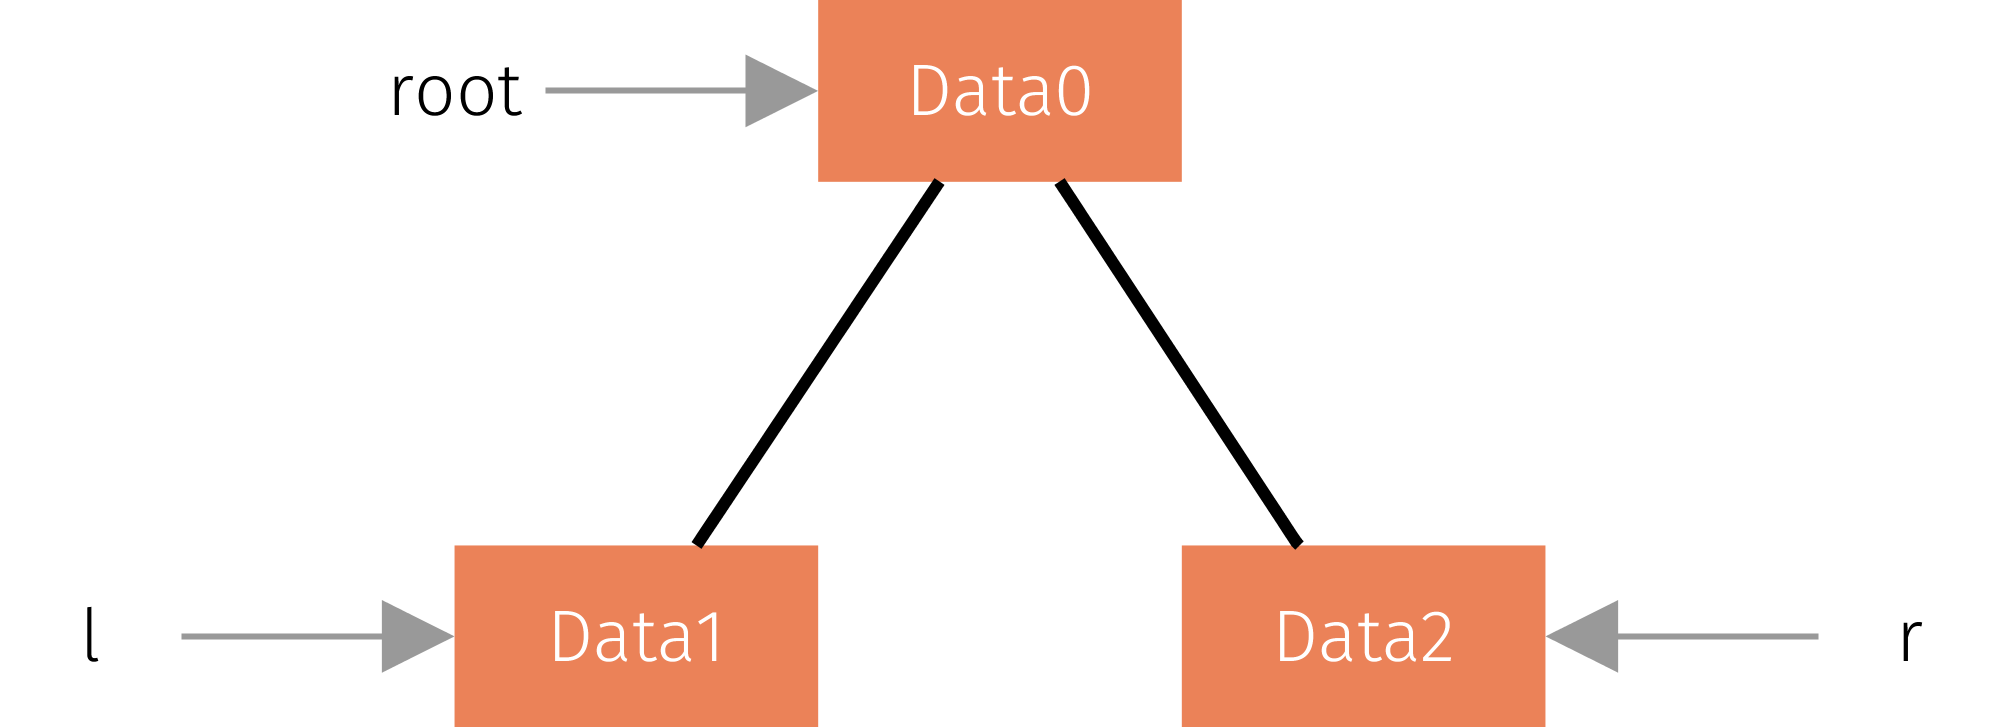
\includegraphics[width=6cm]{img/arbre_bin_4}
    \end{center}
\end{exemple}


\begin{remarque}[]
    Une instance de la classe \mintinline{python}{Node} contient 
    \begin{itemize}
        \item une valeur;
        \item 2 références à 2 autres instances de la classe \mintinline{python}{Node} (ou bien \mintinline{python}{None}).
    \end{itemize}
    Tout comme les listes chaînées, les arbres sont des structures qui se prêtent bien à la récursivité.
\end{remarque}


\begin{exemple}[]
    La taille de l'arbre vide est 0, sinon c'est « 1 plus la taille du sous-arbre gauche plus la taille du sous-arbre droit».
    \begin{center}
        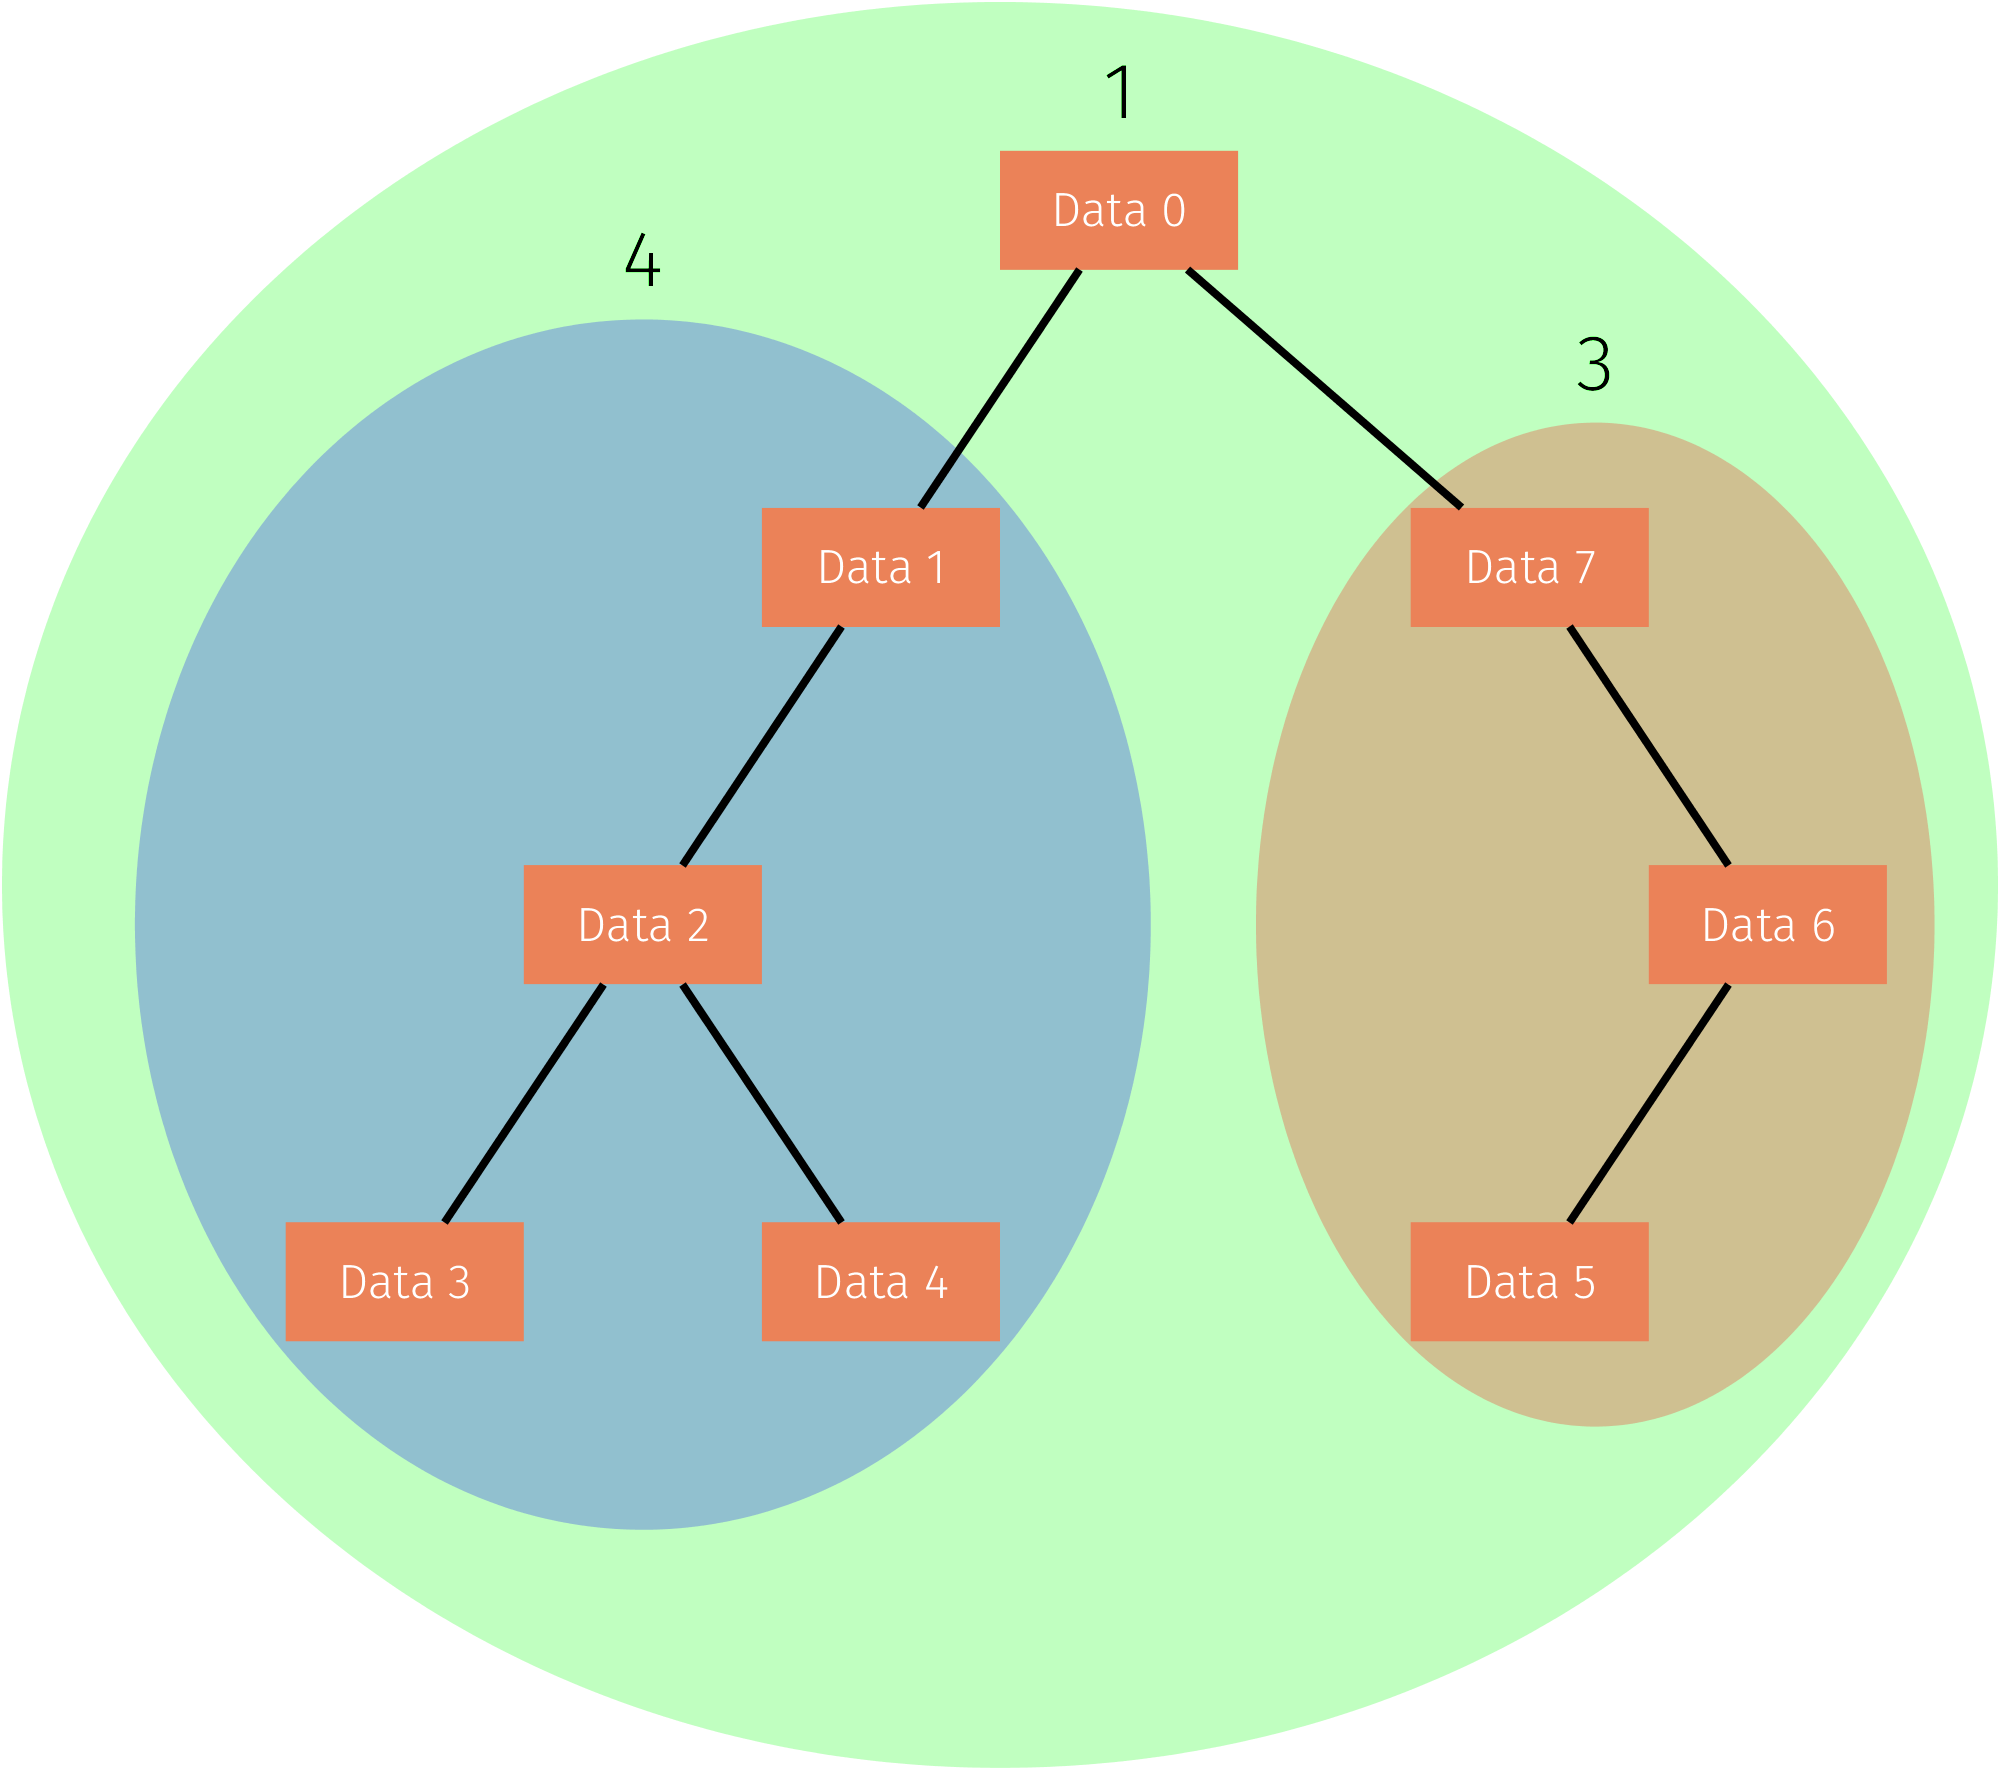
\includegraphics[width=5.5cm]{img/taille}
    \end{center}
    La taille de cet arbre est 1 + 4 + 3 = 8.   
\end{exemple}


\section{Parcours}
\subsection{Différents parcours}
Pour parcourir un arbre binaire, on peut utiliser diverses méthodes récursives.\\
Parmi celles-ci, il en existe qui consistent à\\ 
\begin{itemize}
    \item traiter le n\oe ud courant;\\
    \item parcourir le sous arbre gauche s'il est non vide;\\
    \item parcourir le sous-arbre droit s'il est non vide.\\
\end{itemize}
Et ceci \textit{dans un ordre donné}.\\
Si on choisit de toujours parcourir le sous-arbre gauche avant le droit, cela nous donne 3 méthodes.

\subsection{Préfixe, infixe, postfixe}
\begin{itemize}
    \item \textbf{Parcours préfixe :} Traiter d'abord le n\oe ud courant puis ensuite parcourir le sous-arbre gauche, puis le droit.\\
    \item     \begin{center}
              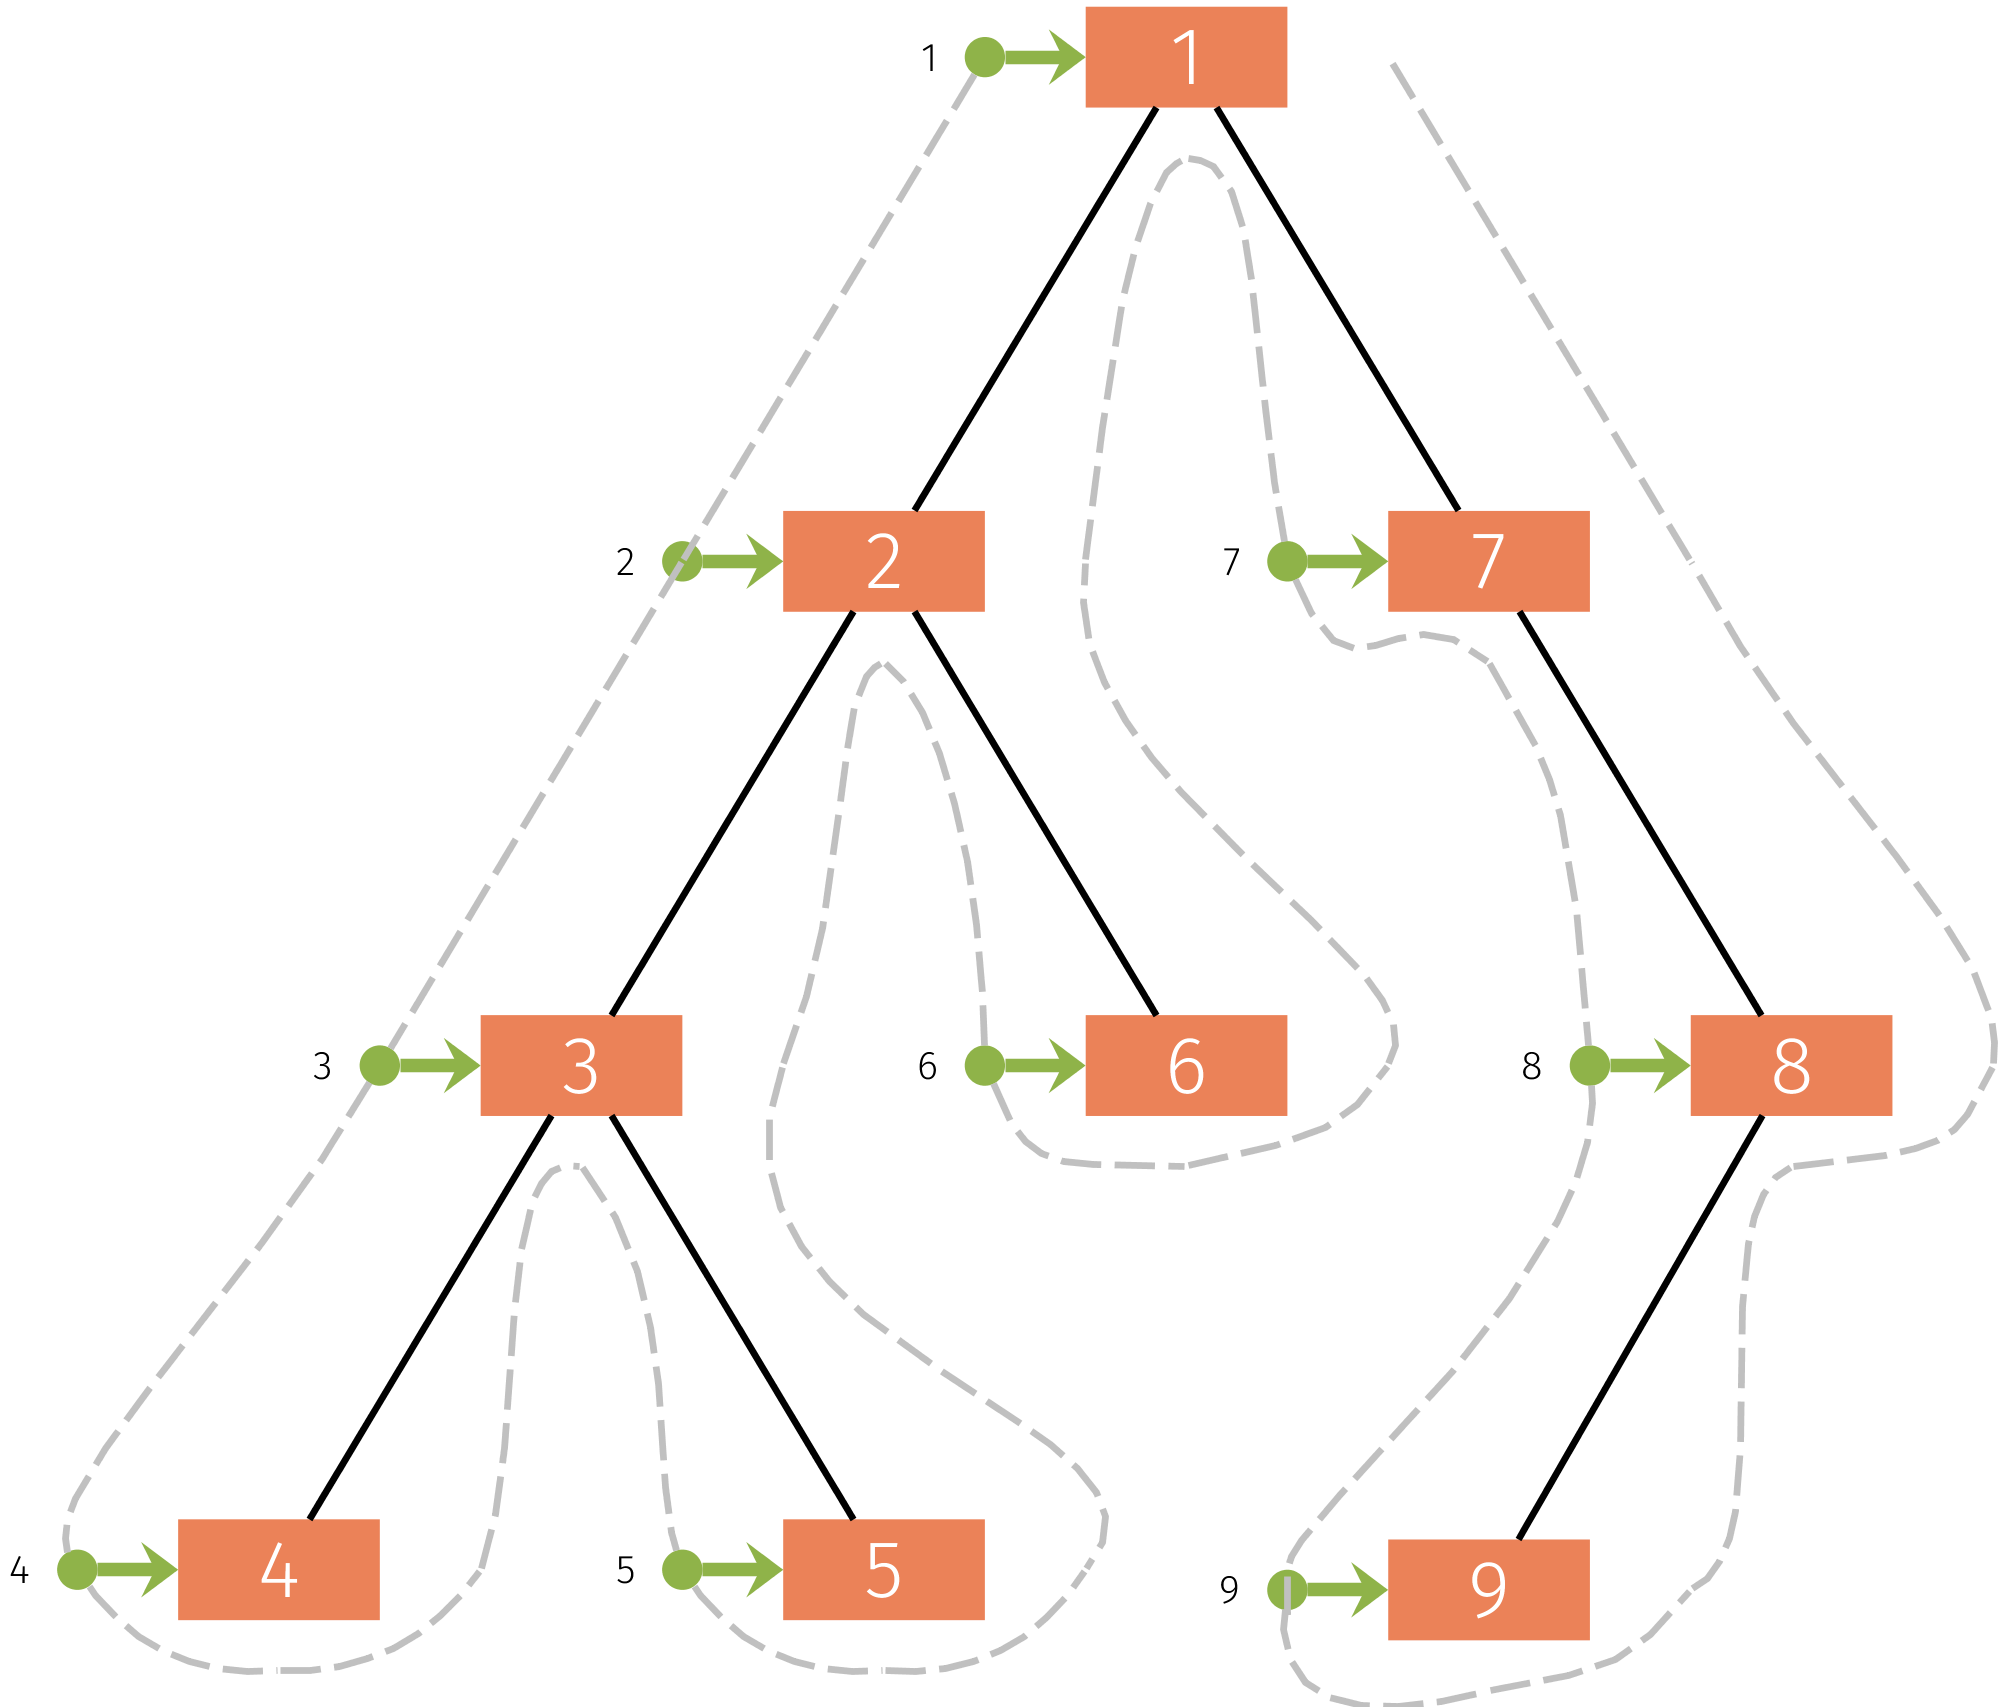
\includegraphics[width=7cm]{img/prefixe.png}
          \end{center}
    \item \textbf{Parcours infixe :} Parcourir d'abord le  sous-arbre gauche, puis traiter le n\oe ud courant et ensuite parcourir le sous-arbre le droit.\\
          \begin{center}
              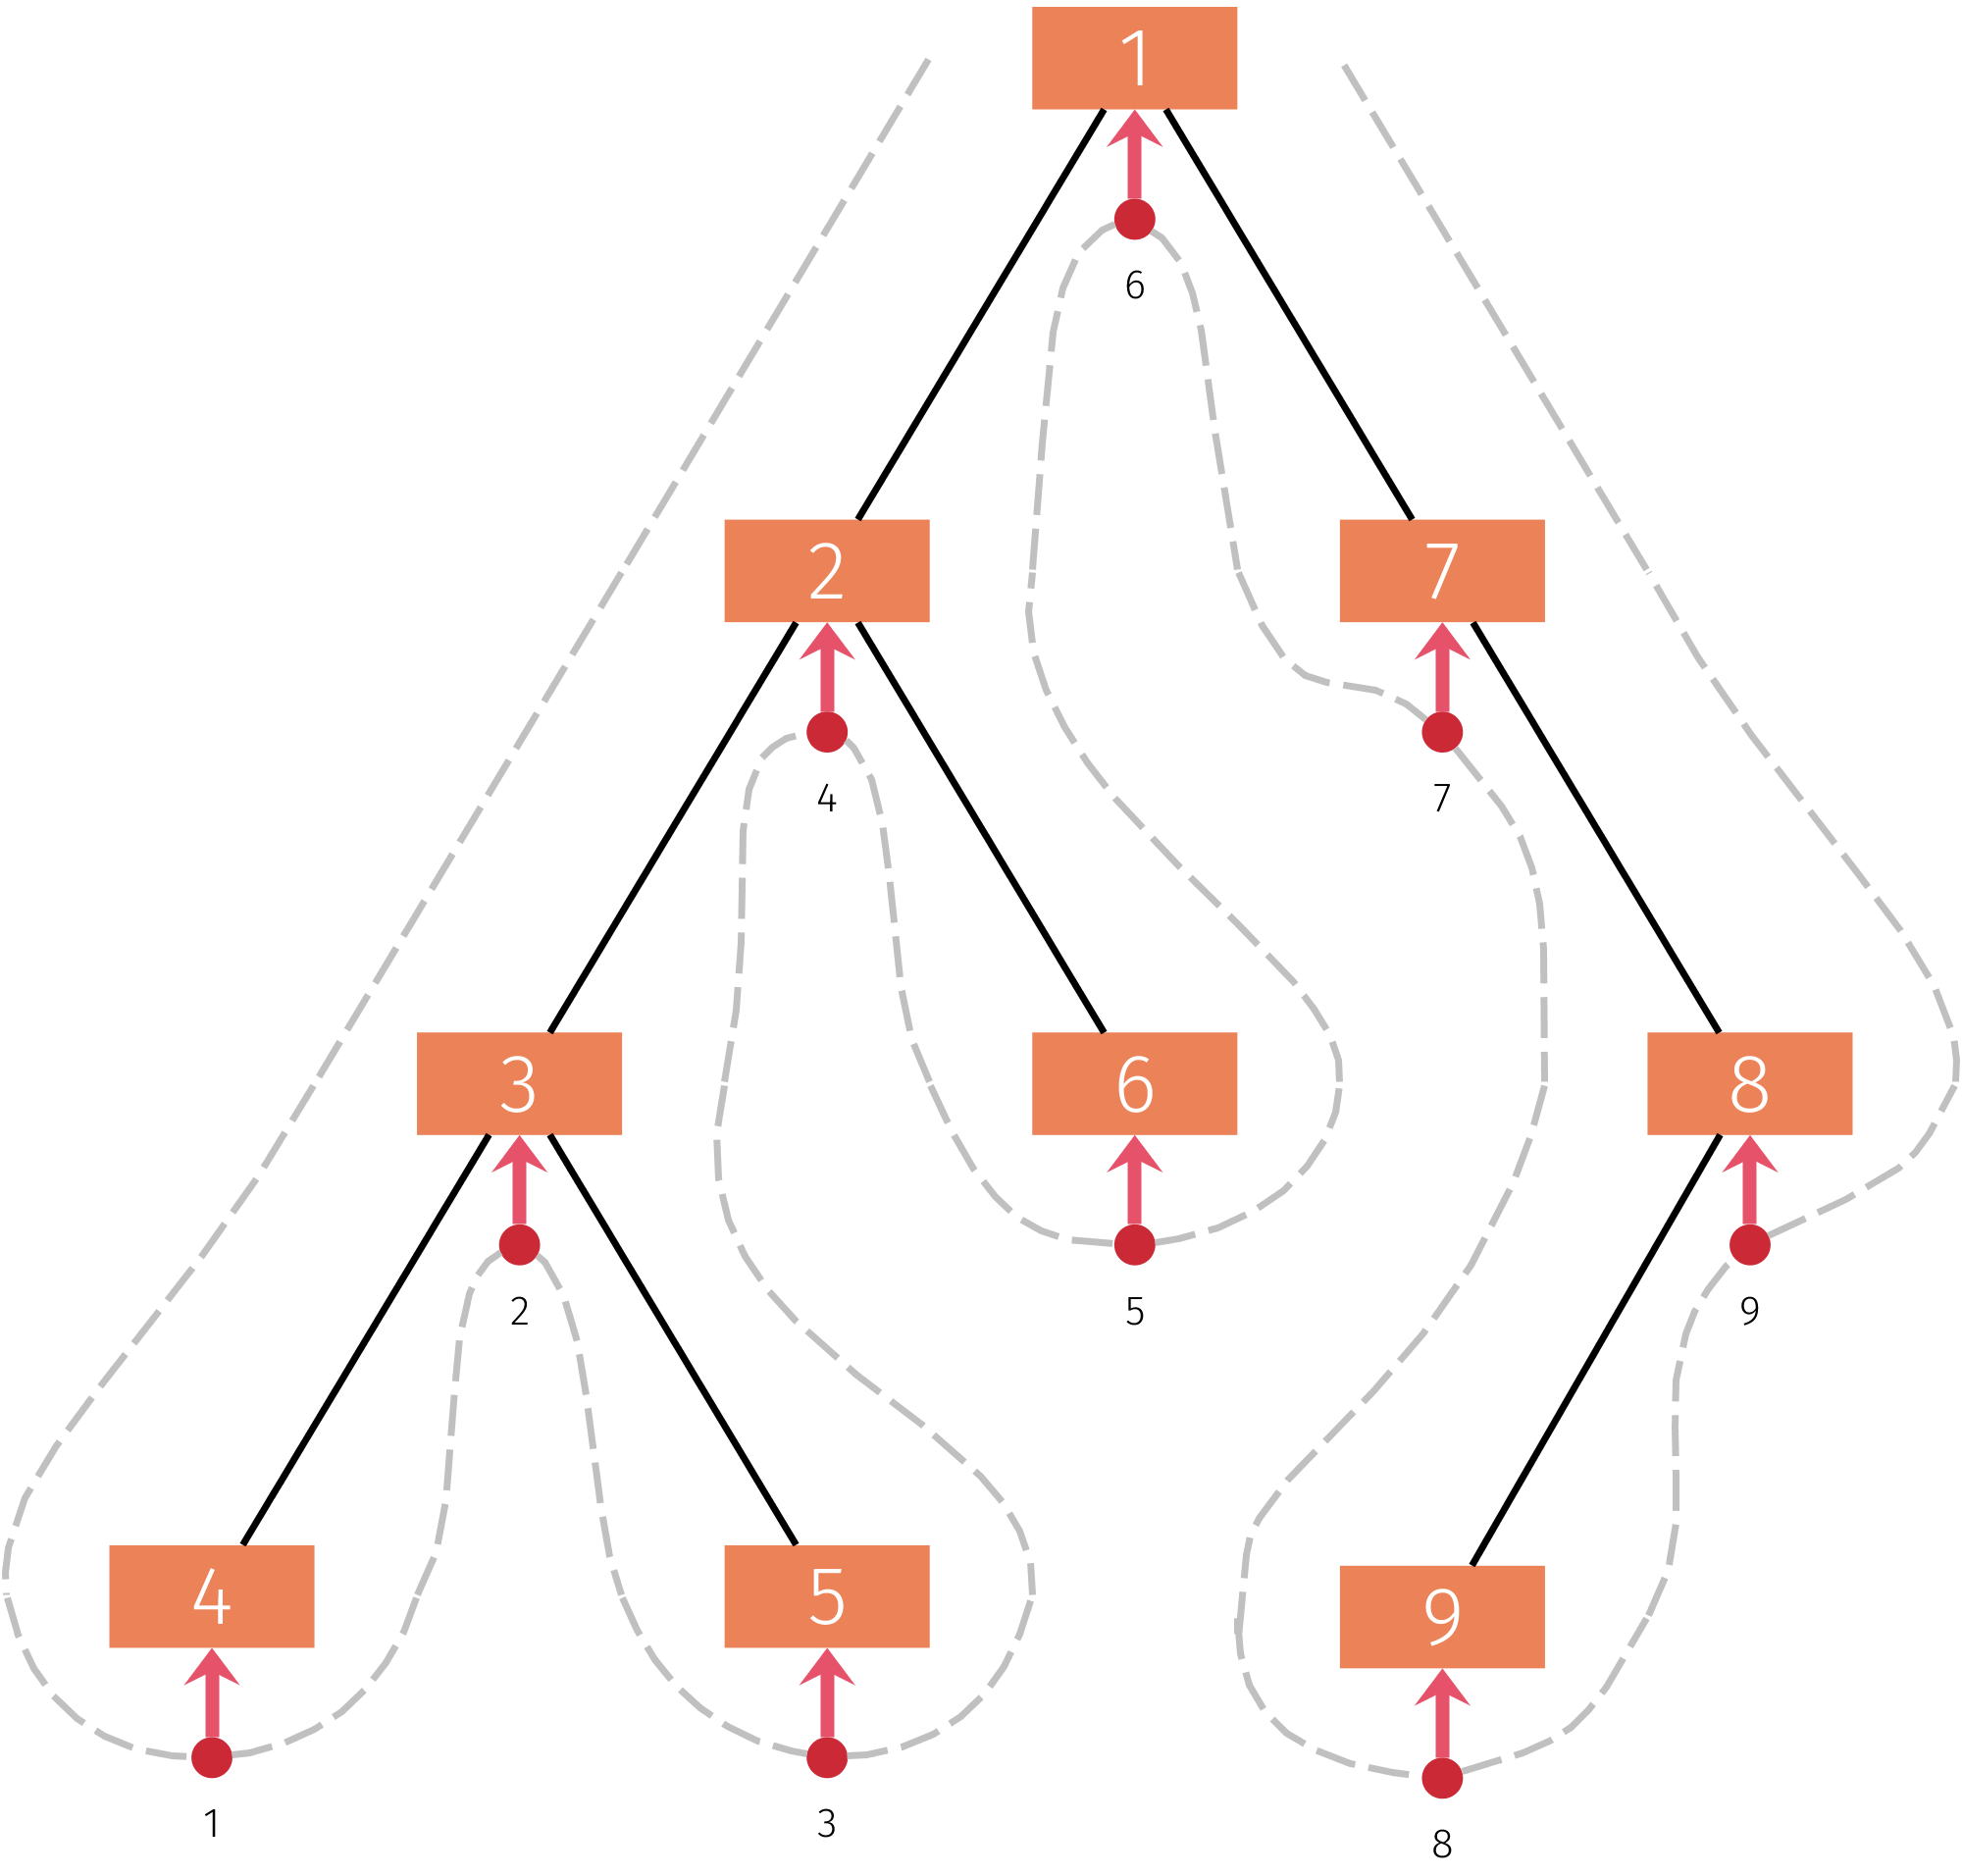
\includegraphics[width=7cm]{img/infixe.png}
          \end{center}
          
    \item  \textbf{Parcours postfixe ou suffixe :} Parcourir d'abord les sous-arbres gauche et droit puis traiter le n\oe ud courant.\\
          \begin{center}
              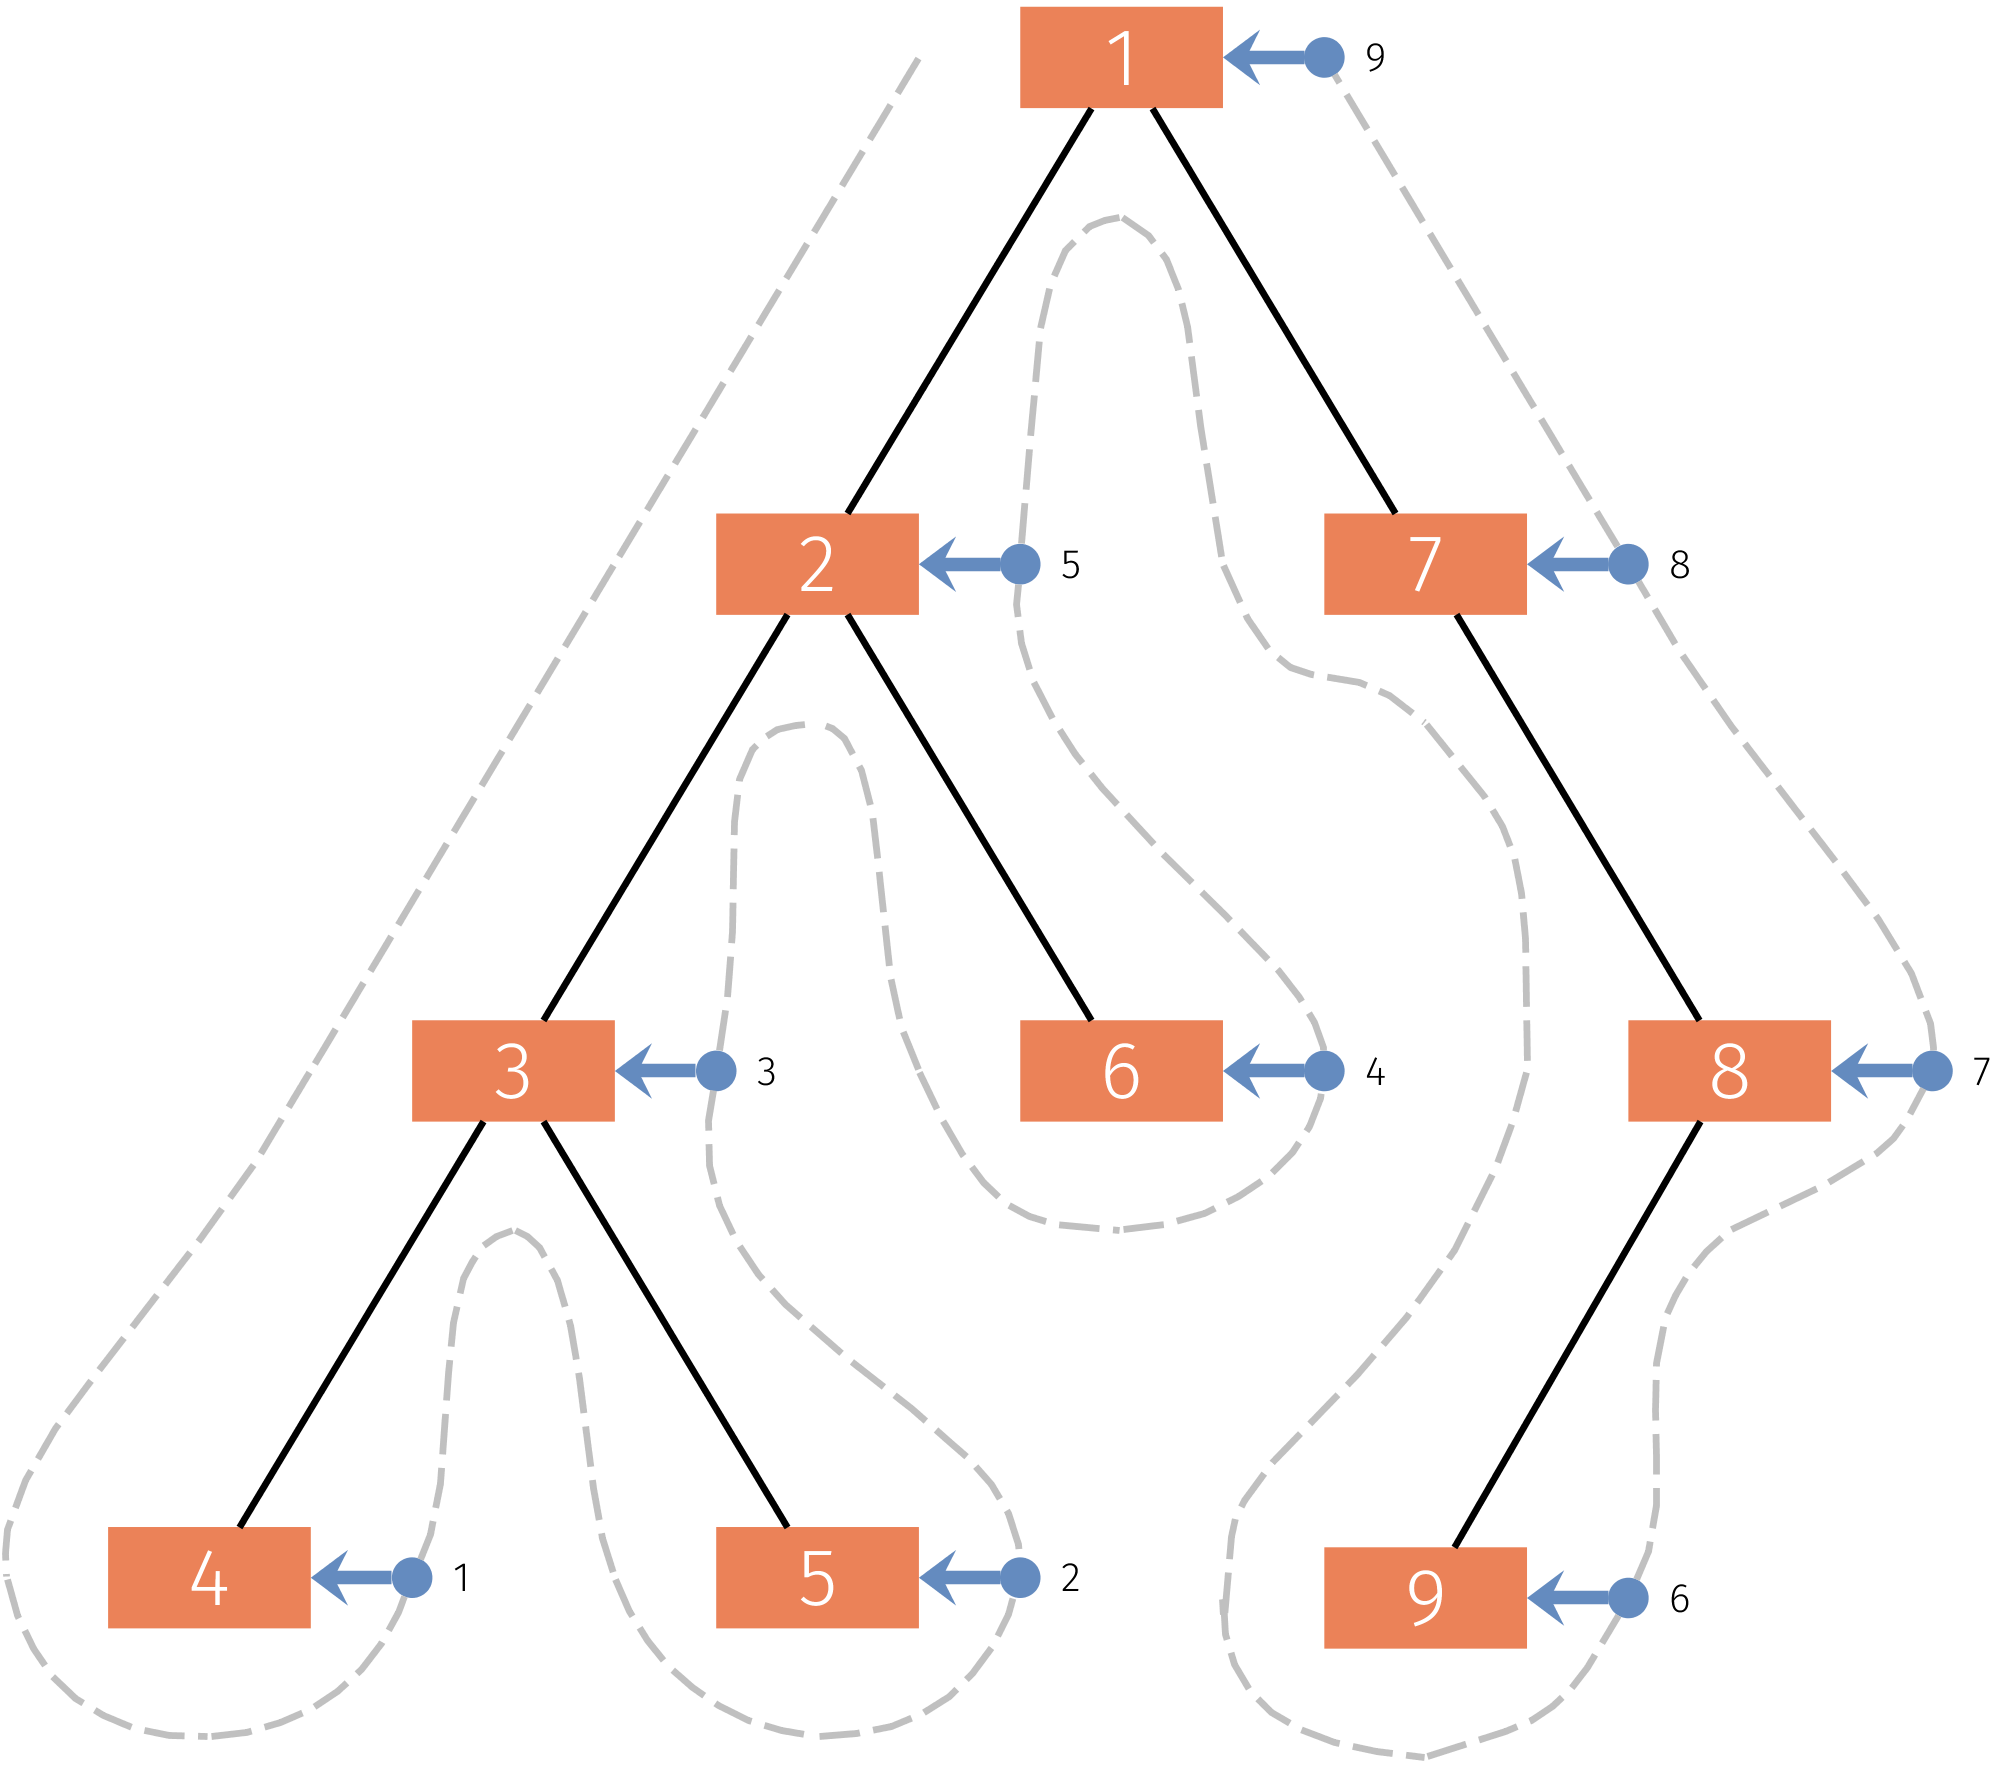
\includegraphics[width=7cm]{img/suffixe.png}
          \end{center}
\end{itemize}
\section{Exercices}

\begin{exercice}[: construire des arbres]
    \begin{enumerate}
        \item   Dessiner tous les arbres binaires de taille 2.
        \item   Dessiner tous les arbres binaires de taille 3.
    \end{enumerate}
\end{exercice}


\begin{exercice}[: dénombrer des arbres]
    Sachant qu'il existe
    \begin{itemize}
        \item 1 arbre vide;
        \item 1 arbre de taille 1;
        \item 2 arbres de taille 2;
        \item 5 arbres de taille 3;
        \item 14 arbres de taille 5.
    \end{itemize}
    Déterminer sans les construire le nombre d'arbres de taille 5.
\end{exercice}
\begin{exercice}[: une relation entre la hauteur et la taille d'un arbre]
    Soit h un entier naturel et A un arbre de hauteur h.
    \begin{enumerate}
        \item Combien, au minimum, A possède-t-il de n\oe uds ?
        \item Combien, au maximum, A possède-t-il de n\oe uds ?
    \end{enumerate}
    
    On en déduit l'encadrement suivant :\\
    soit N la taille d'un arbre de hauteur h, alors on a 
    $$\Large\fbox{\hspace{3em}\leq N \leq\hspace{3em}}$$
\end{exercice}

\begin{exercice}[: Parcours « à la main»]
    \begin{center}
        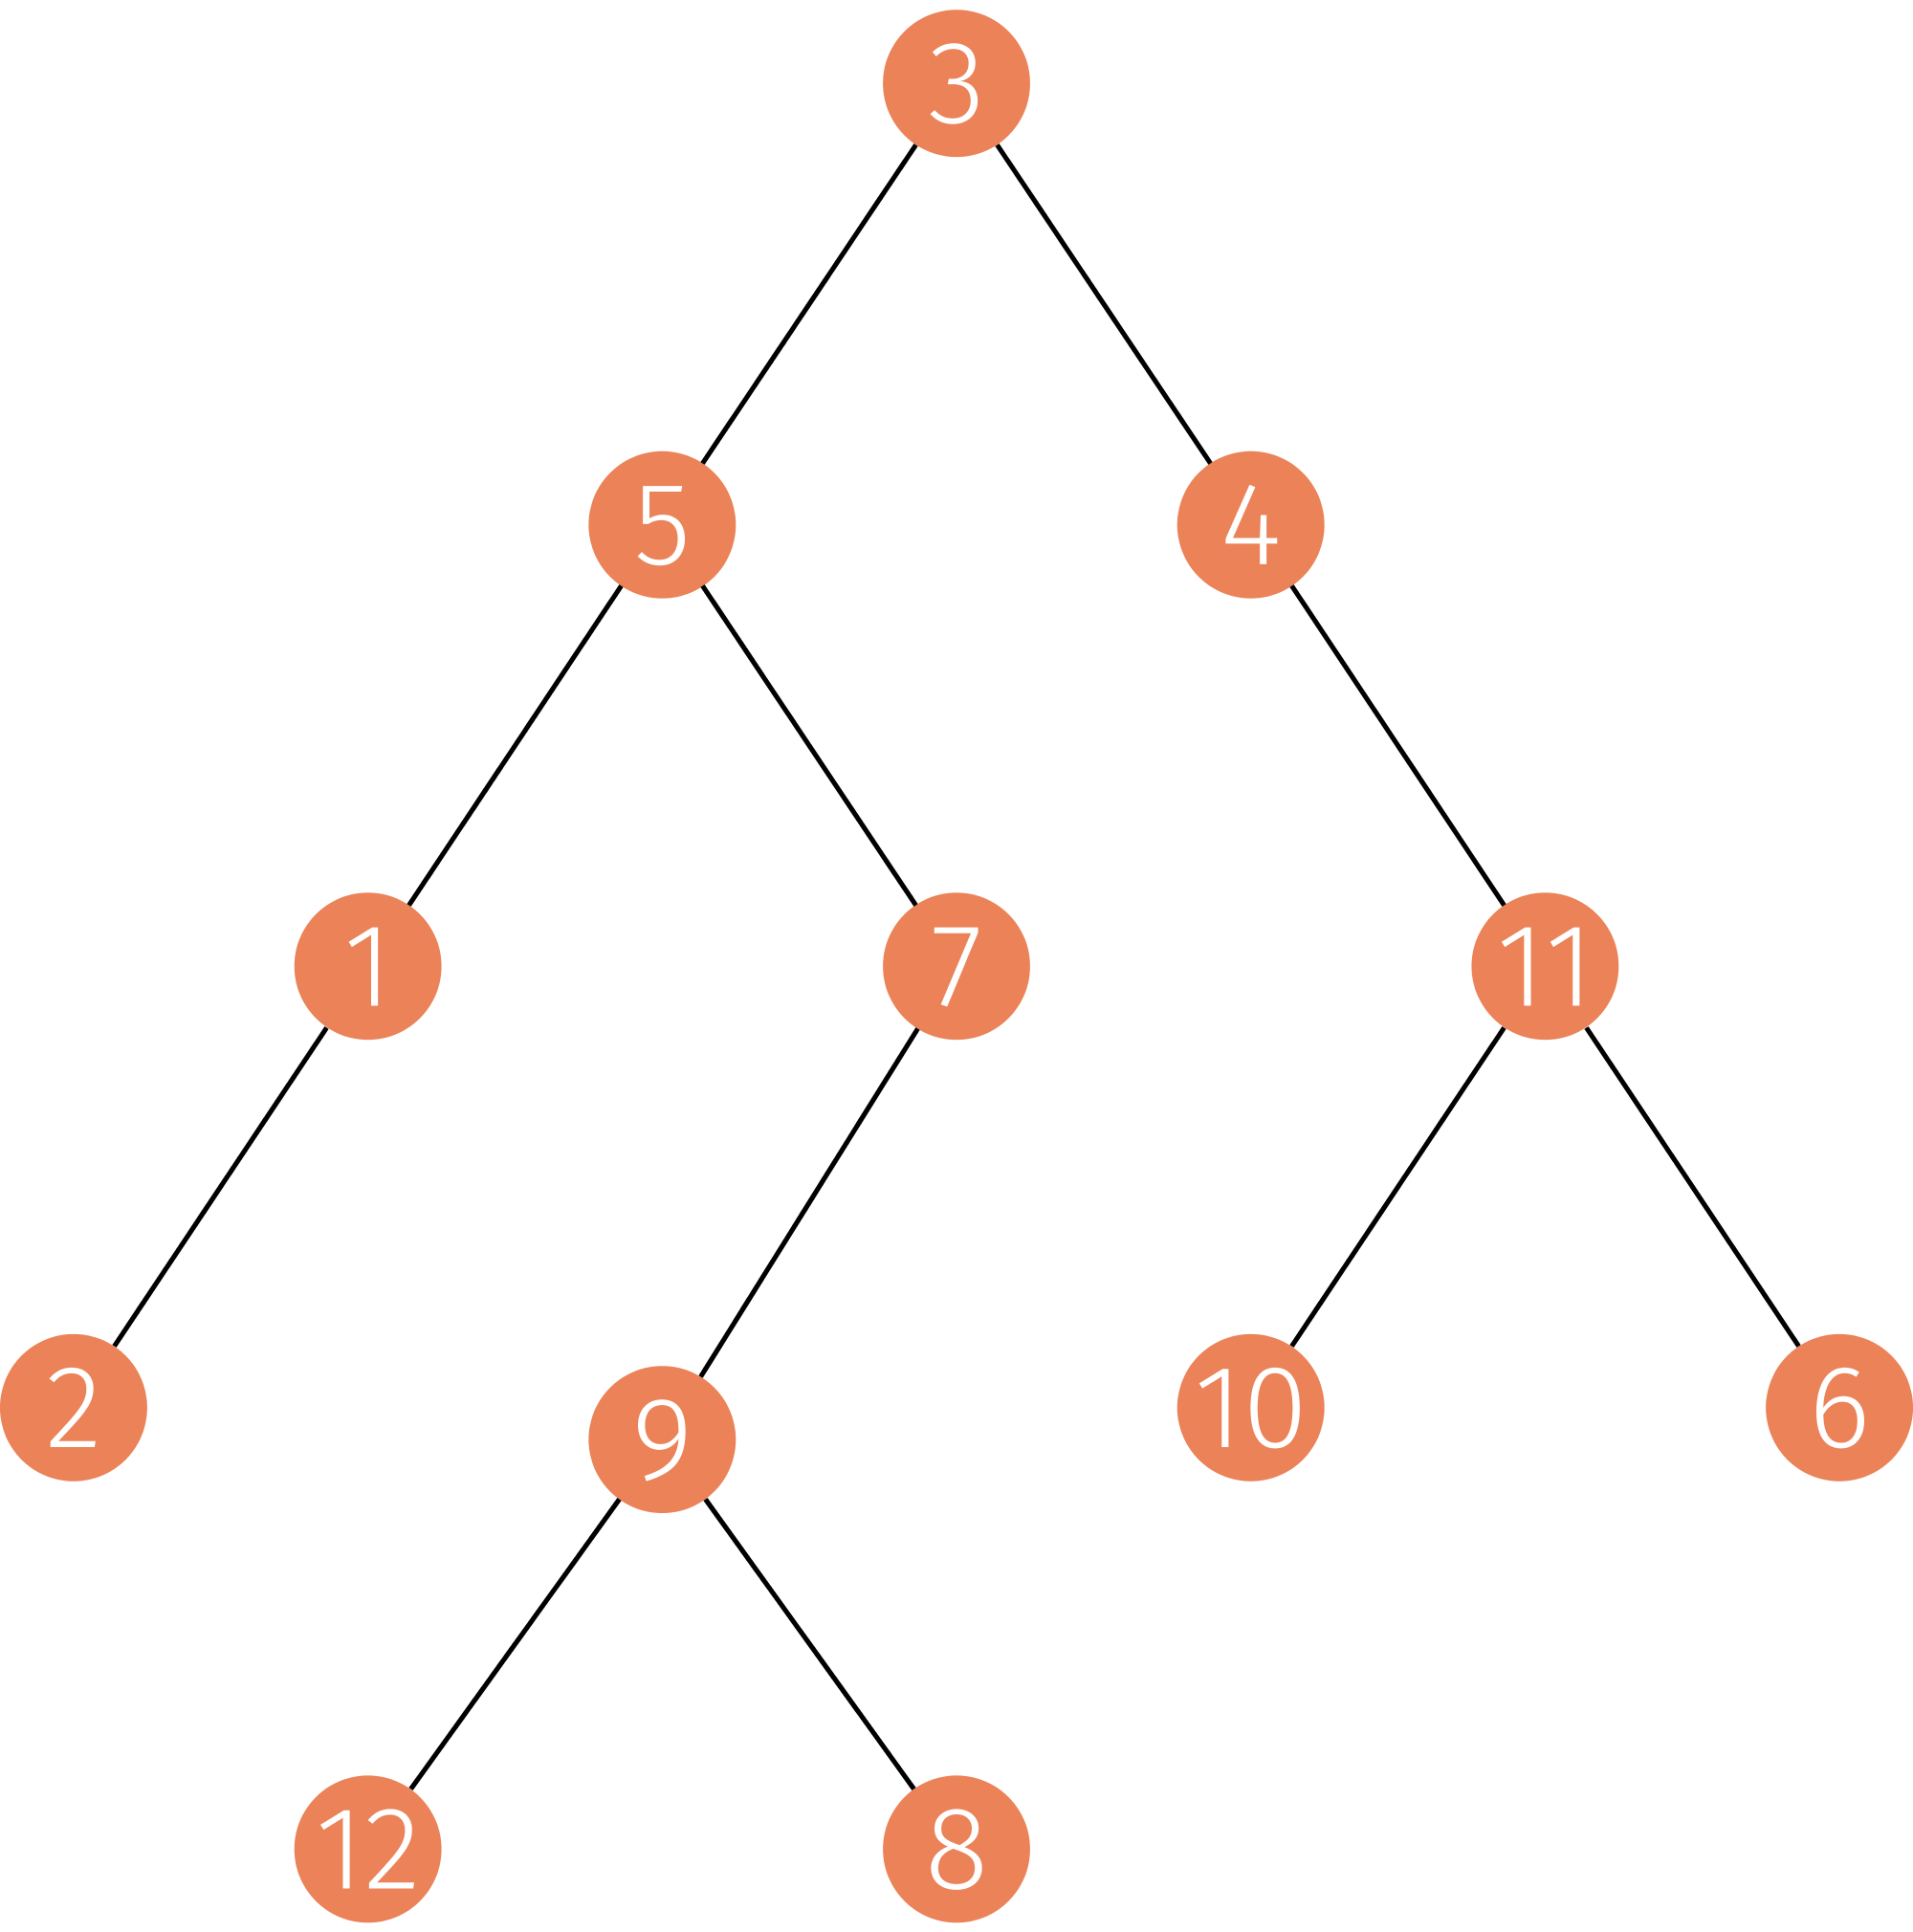
\includegraphics[width=7cm]{img/arbre2}
    \end{center}
    \begin{enumerate}
        \item \'Ecrire les valeurs de l'arbre dans l'ordre de son parcours préfixe.
        \item Faire de même avec un parcours infixe.
        \item Faire de même avec un parcours postfixe.
    \end{enumerate}
\end{exercice}

\begin{exercice}
    \begin{enumerate}
        \item Créer un fichier \texttt{Node.py} et implémenter la classe \texttt{Node} vue en cours.
        \item Implémenter la méthode \mintinline{python}{__str__} qui  utilise une sous-fonction récursive  qui :
              \begin{itemize}
                  \item si on lui demande d'afficher \mintinline{python}{None} renvoie \mintinline{python}{''};
                  \item sinon (c'est qu'elle doit bien afficher un n\oe ud)  ouvre une parenthèse, affiche récursivement le sous-arbre gauche, puis  affiche la valeur du n\oe ud, le sous-arbre droit et enfin ferme la parenthèse.\\
              \end{itemize}
              sur l'arbre suivant
              \begin{center}
                  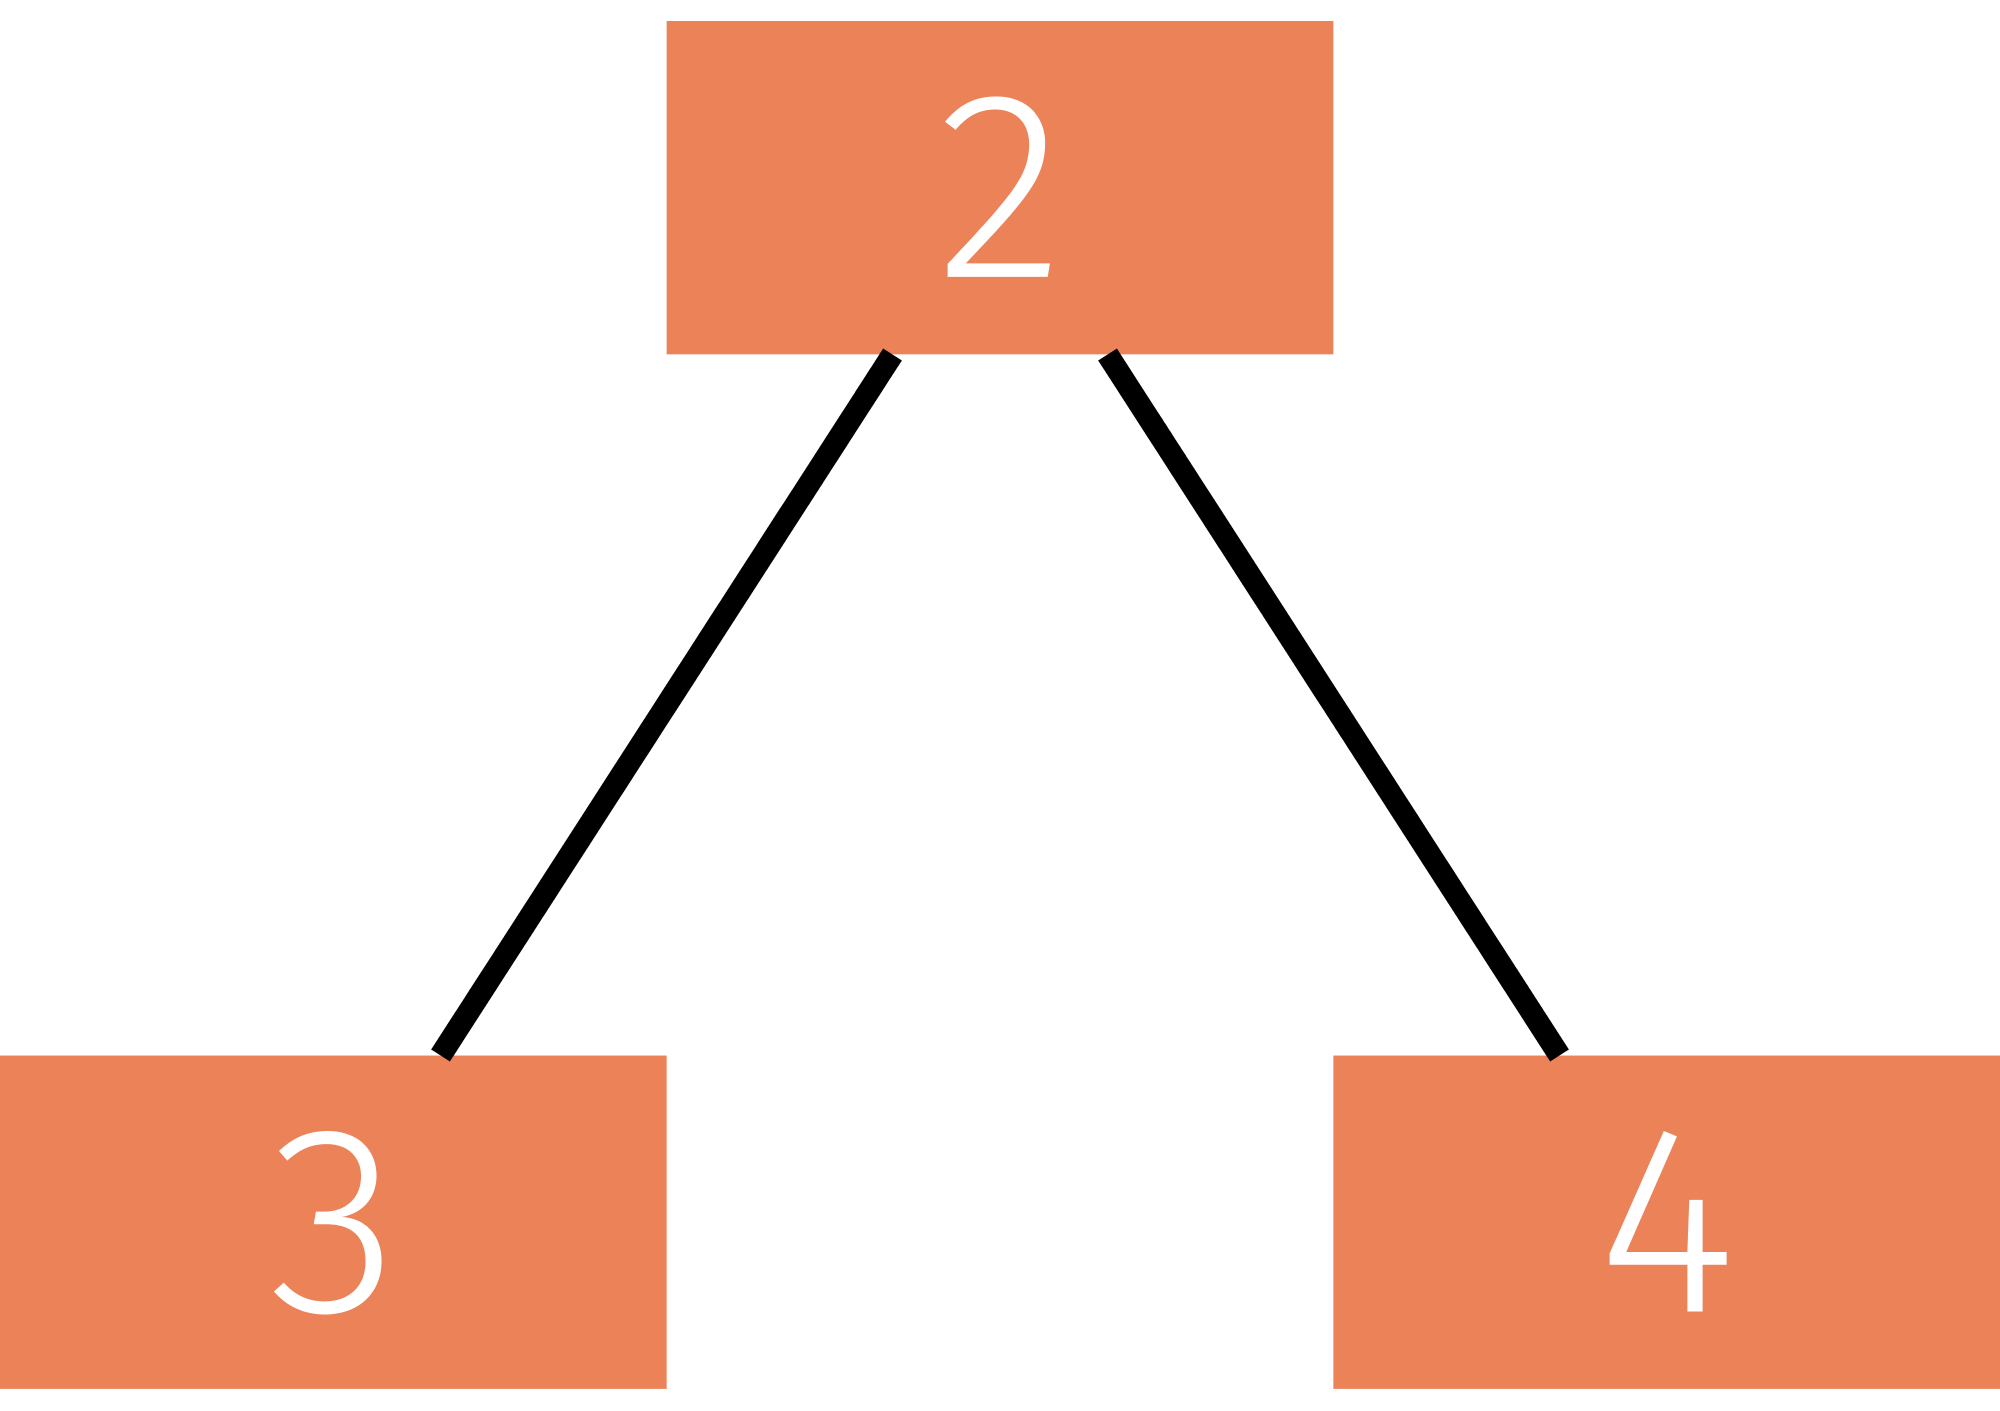
\includegraphics[width=3cm]{img/arbre1.png}
              \end{center}
              qui est créé par
              \begin{minted}{python}
    a = Node(3)
    b = Node(4)
    c = Node(2, a, b)
    \end{minted}
              \mintinline{python}{print(c)} devra renvoyer \mintinline{python}{'((3)2(4))'}
        \item Implémenter la méthode d'instance \mintinline{python}{size} qui renvoie un \mintinline{python}{int} qui est la taille de l'arbre (s'aider du cours).
        \item Comment trouver récursivement la hauteur d'un arbre ? Proposer une « méthode logique» et implémenter la méthode d'instance \mintinline{python}{height}, qui renvoie un \mintinline{python}{int} qui est la hauteur de l'arbre.
        \item Implémenter la méthode d'instance \mintinline{python}{__eq__} qui renvoie \mintinline{python}{True} si deux arbres sont égaux et \mintinline{python}{False} sinon (trouver une méthode récursive).
    \end{enumerate}
\end{exercice}
\begin{exercice}[: Parcours]
    \begin{enumerate}
        \item Ajouter à la classe \mintinline{python}{Node} une méthode d'instance \mintinline{python}{prefix} qui renvoie un \mintinline{python}{str} qui est la chaîne de caractères obtenue en concaténant toutes les valeurs des n\oe uds de l'arbre au cours de son parcours préfixe.
        \item De même implémenter \mintinline{python}{infix} et \mintinline{python}{postfix}.
    \end{enumerate}
\end{exercice}
\end{document}